\begin{figure*}[h!]
    \centering
    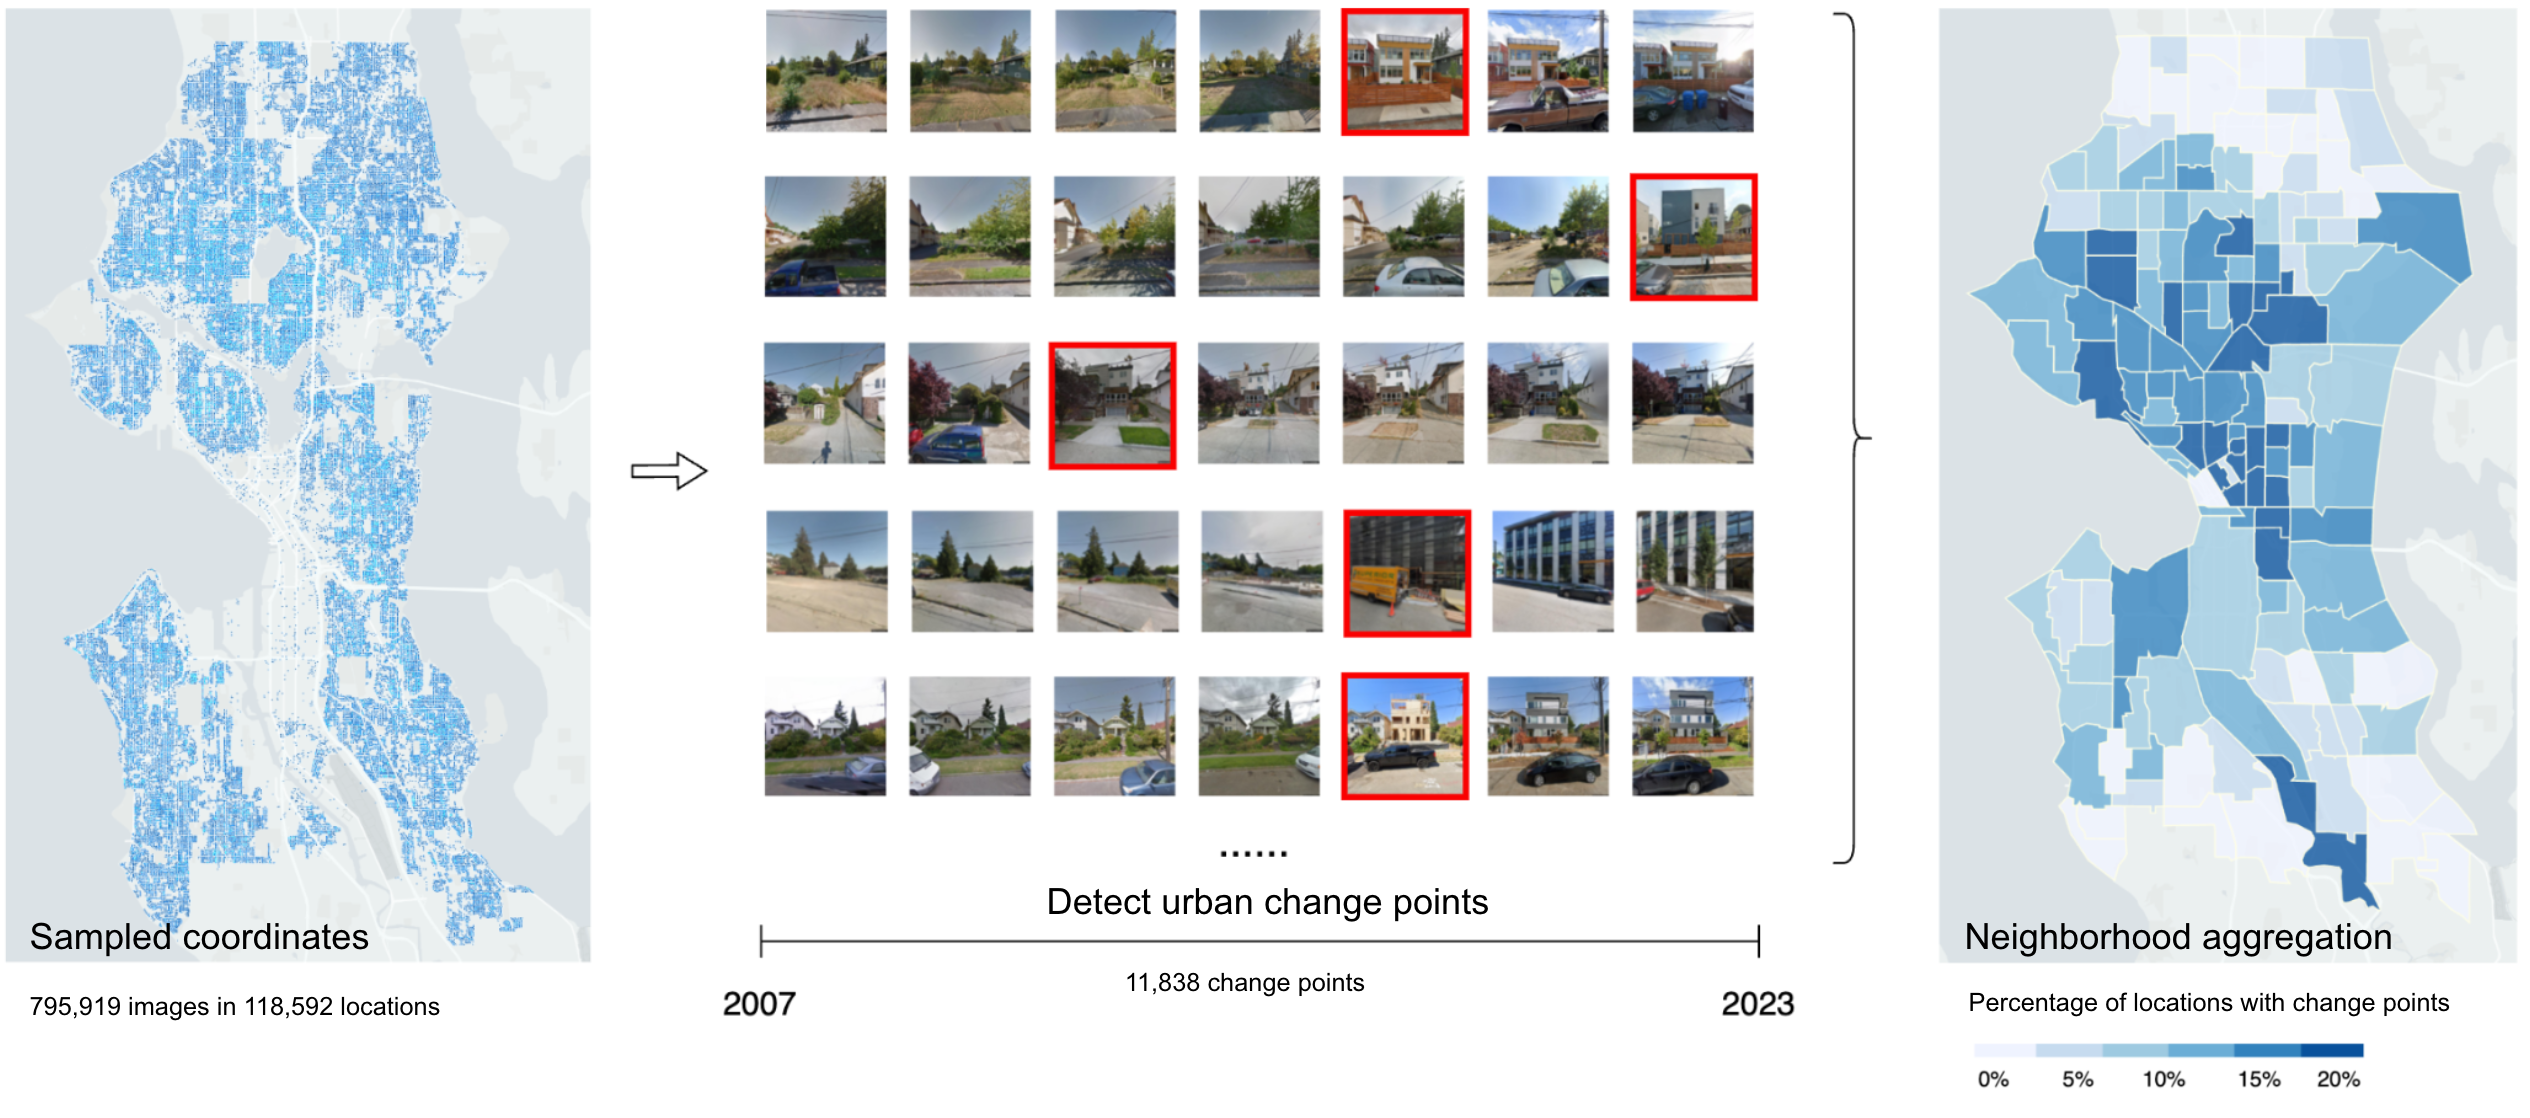
\includegraphics[width=1.01\linewidth]{figure/seattle.png}
    \caption{Assessing urban change in Seattle. \textbf{Left:} Location of approximately $800$k sampled street view images, each represented by a blue dot. \textbf{Middle:} Results from deploying our change detection model on the sampled images to pinpoint urban changes shown in red bounding boxes. \textbf{Right:} Change points, aggregated at the census tract level, with color denoting the proportion of street view time series that have been identified as change.}
    \label{fig:seattle}
\end{figure*}


% \begin{figure*}[h!]
%     \centering
%     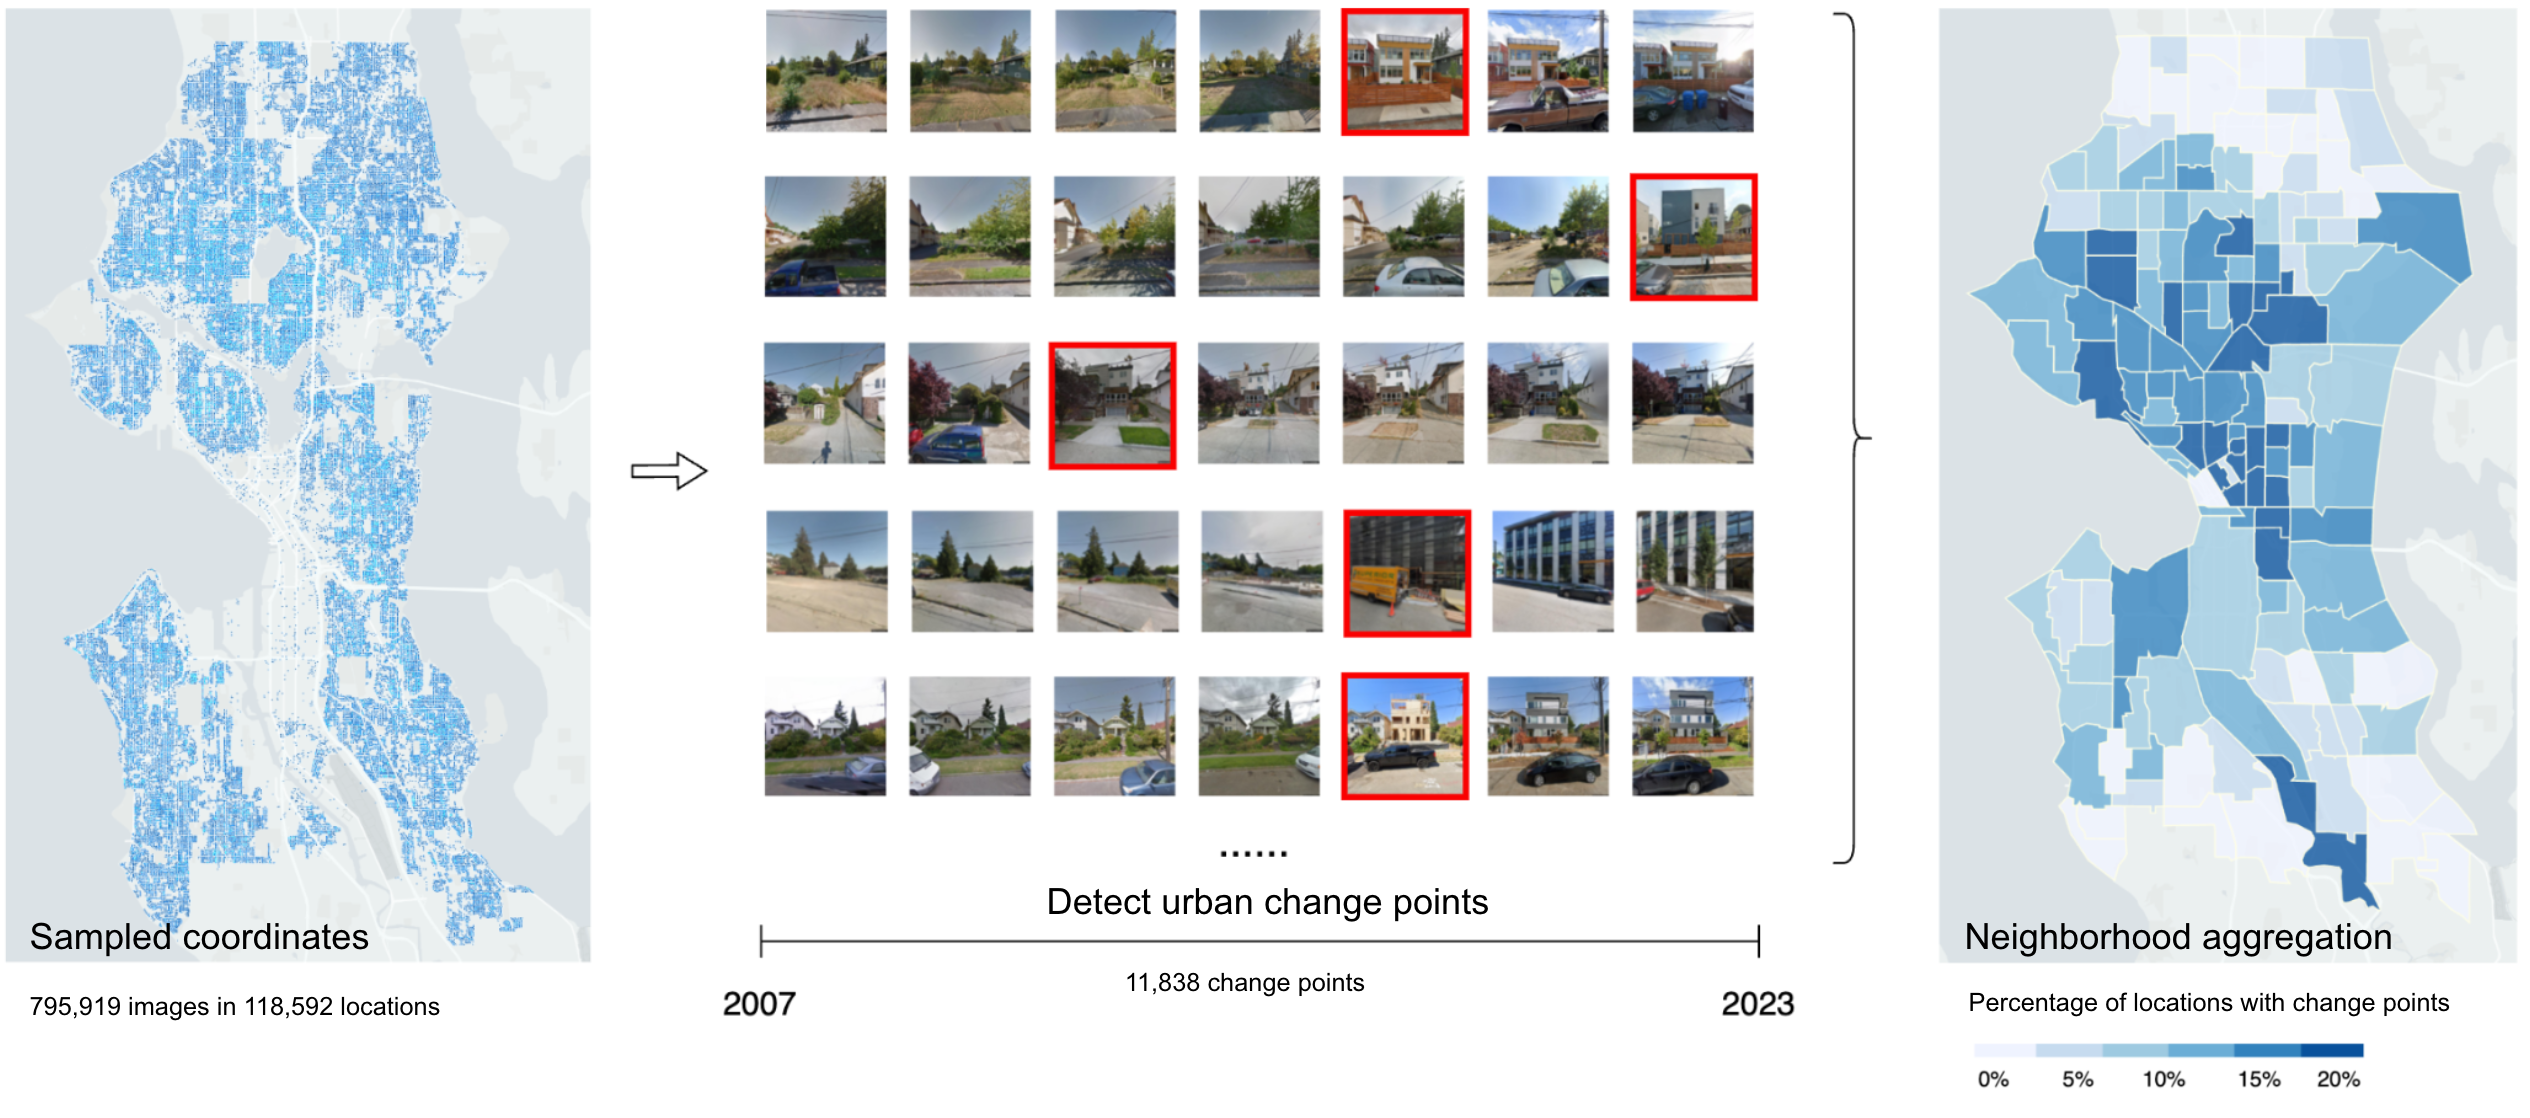
\includegraphics[width=1.01\linewidth]{figure/seattle.png}
%     \caption{Assessing urban change in Seattle. \textbf{Left:} We sampled around $800k$ street view images in total and each blue dot indicates its location. \textbf{Middle:} Applying our proposed change detection model directly on all sampled images and identify urban change points. \textbf{Right:} Aggregating detected change points to the census tract level, the color indicates the percentage of sampled time series detected with urban change points.}
%     \label{fig:seattle}
% \end{figure*}